\documentclass[utf8]{article}
\usepackage[a4paper, total={6in, 8in}]{geometry}

\usepackage{interval}
\intervalconfig{soft open fences}
\usepackage{natbib}
\usepackage{lineno}
\linenumbers
% import Eq and Section references from the main manuscript where needed
\usepackage{xr}
\externaldocument{manuscript}
% \externaldocument{methods}
\externaldocument{supplementary}

\newcommand{\linerange}[2]{%
\ifthenelse{\equal{\getrefnumber{#1}}{\getrefnumber{#2}}}{%
line \ref{#1}%
}{%
lines \ref{#1}--\ref{#2}%
}%
}
% package needed for optional arguments
\usepackage{xifthen}
\renewcommand{\thefigure}{R\arabic{figure}}

\usepackage{url,hyperref,lineno,microtype}

\usepackage[onehalfspacing]{setspace}
\usepackage{graphicx}
\usepackage{amsmath}
\usepackage{cleveref}
\usepackage{physics}
\usepackage{siunitx}
\usepackage{xr}
\usepackage{bm}
\usepackage{cases}

\graphicspath{{../figures/}}

\setcounter{section}{0}
\newcounter{point}[section]
\setcounter{point}{0}

% command declarations for reviewer points and our responses

\newenvironment{point}
{\refstepcounter{point} \bigskip \noindent {\textbf{Point~P\thesubsection.\arabic{point}} } ---\ }
{\par }

\newcommand{\shortpoint}[1]{\refstepcounter{point}  \bigskip \noindent
	{\textbf{Point~P\thesubsection.\arabic{point}} } ---~#1\par }

\newenvironment{reply}
{\medskip \noindent Reply:\  }
		{\medskip}

\newcommand{\shortreply}[2][]{\medskip \noindent Reply:\  #2
		\ifthenelse{\equal{#1}{}}{}{ \hfill \footnotesize (#1)}%
		\medskip}


\begin{document}
% \onecolumn
% \firstpage{1}

\begin{center}
	\Large Response to the reviewers
\end{center}
We are very grateful to the reviews for their comments.
We are, of course, very pleased that Reviewer 2 was so supportive of our manuscript and that they have endorsed publication.
We were equally pleased that Reviewer 1 has engaged so fully with our work, that they saw value in our results and have provided such thoughtful and valuable suggestions.
We are sorry it has taken a long time to reply; we wanted to give careful consideration to these suggestions and have made a number of substantial extensions to the work which we believe has made it stronger; we are very grateful for the help the referee comments provided in this.

The biggest changes in the revised manuscript came as a result of points \hyperref[p:biol]{P2.1.1} and \hyperref[p:gstar]{P2.3.8}, which led us to revert our model to the original equations and parameter values used in \cite{bose2011}.
The motivation behind a slightly different model in our original manuscript, as well as the consequence of the latest changes in the revised manuscript, are explained in \cref{sec:model}.
Both reviewers also pointed out that some of our notation and terminology is unclear.
As a result we renamed many of the terms, an overview of the most important terms is given in \cref{sec:terminology}.
We will refer to the first version of the manuscript that was submitted to the journal as the ``original manuscript'' (M0), and we will call the latest submitted version the ``revised manuscript'' (M1).
If not otherwise stated, the equations numbers, figures, and line numbers refer to the revised manuscript.
This response is structured as follows:
\Cref{sec:sum} contains the terminology as well as summarises the main model changes in the revised manuscript.
In \cref{sec:r1} we address the concerns raised by Reviewer 1, and in \cref{sec:r2} the concerns raised by Reviewer 2.


\section{Summary of changes}
\label{sec:sum}

\subsection{Terminology and notation}
\label{sec:terminology}
Notation and terminology in this field is surprisingly controversial; different authors use different terms for the same thing and the same terms for things that are different, sometimes subtly different.
We have tried to follow the referees suggestions as much as possible, but would be grateful for any further guidance.
Below we briefly define the controversial terms.
In the context of a spiking limit cycle of an uncoupled Morris-Lecar (ML) cell we have:
\begin{itemize}
\item $T_{a}$: The time interval when the voltage is above firing threshold, i.e. when $v>v_{\theta}$.
\item $T_{s}$: The time interval when the voltage is below firing threshold, i.e. when $v<v_{\theta}$.
\end{itemize}
In the context of a stable $n:n$ solution we have:
\begin{itemize}
\item \textbf{Active cell}: Cell that is currently firing.
\item \textbf{Silent cell}: Cell that is currently suppressed and does not fire.
\item \textbf{Active phase}: Time interval between the start of the limit cycle and the time when the voltage of the active cell falls below firing threshold after the $n$th spike, i.e. for $t \in \left[0, (n-1)T + T_{a}\right]$.
\item \textbf{Silent phase}: Time interval after the end of the active phase and the cycle period, i.e. for $t \in \interval[open left]{(n-1)T+T_{a}}{P}$
\item \textbf{Active phase map}: Map $F_{n}$ that models the evolution of $d$ during the active phase.
\item \textbf{Recovery phase map}: Map $Q_{n}$ that models the evolution of $d$ during the silent phase.
\item \textbf{Left and right branch borders}: The left and right branch borders of stable $n:n$ solutions are denoted by $\bar g_{\mathcal{L}}(n)$ and $\bar g_{\mathcal{R}}(n)$, respectively.
\end{itemize}

\subsection{Model changes}
\label{sec:model}
% Overview
In this section we first explain the model differences between the \cite{bose2011} paper and our original manuscript.
We will then outline a short motivation for these changes.
Finally the model of the revised manuscript is discussed.
There are two main differences in the model equations and parameters between the original manuscript and \cite{bose2011}:
First, the value of the applied current $I$ is different: In \cite{bose2011} they have $I=3.8$ $\si{\mu A/cm^2}$, in the original manuscript we had $I=6$ $\si{\mu A/cm^2}$.
Second, the original manuscript uses step-wise resets of $d$ and $s$ to simplify the dynamics of the active state of the spike (when $v > v_{\theta}$).

\begin{figure}[h!]
	\centering
	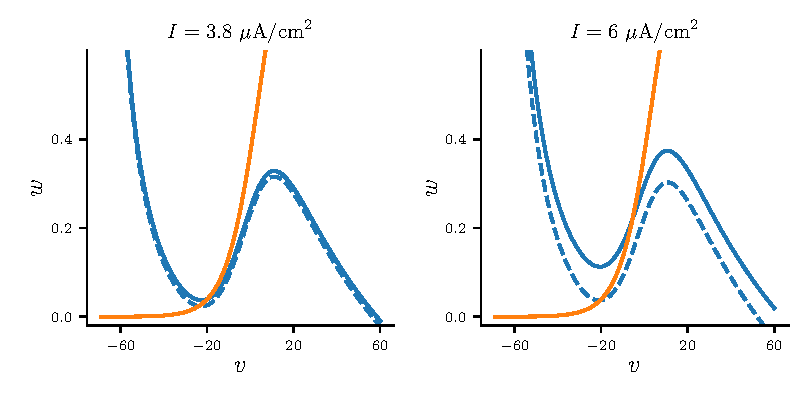
\includegraphics[width=0.9\textwidth]{model-changes}
	\caption{Nullclines of the \cite{bose2011} ML model with $I=3.8$ $\si{\mu A/cm^2}$ (left), and the model from our original manuscript with $I=6$ $\si{\mu A/cm^2}$ (right). The solid blue lines are the $v$-nullclines when $\bar g s=0$. The dashed blue lines are the $v$-nullclines when $\bar g s$ is near the respective bifurcation point where the fixed point changes stability.\label{fig:nullclines}}
\end{figure}

The main motivation for increasing $I$ in the original manuscript had to do with the ``excitability'' of a silent ML cell, and was to simplify the explanation of the concept of the ``release conductance''.
\Cref{fig:nullclines} shows the $v$- and $w$-nullclines for $I=3.8$ $\si{\mu A/cm^2}$ (left) and for $I=6$ $\si{\mu A/cm^2}$ (right) when no inhibition is applied and $g = 0$ (let $g:= \bar g s$).
The dashed lines indicate the $v$-nullcline at the bifurcation point when the total synaptic conductance $g$ is at the respective bifurcation value, $g=g_{bif}$.
In case of $I=3.8$ $\si{\mu A/cm^2}$ we have $g_{bif}\approx 0.007$ $\si{\mu A/cm^2}$, whereas for $I=6$ $\si{\mu A/cm^2}$ we have $g_{bif}\approx 0.03804$ $\si{\mu A/cm^2}$.
Hence for $I=3.8$ $\si{\mu A/cm^2}$ and $g=0$, the unstable fixed point is ``closer'' in phase space to the stable fixed point at bifurcation when $g=g_{bif}$, than in case of $I=6$ $\si{\mu A/cm^2}$.
In other words, a silent cell with $I=3.8$ $\si{\mu A/cm^2}$ is ``easier to excite'' than a silent cell with $I=6$ $\si{\mu A/cm^2}$.

In contrast to the $I=6$ $\si{\mu A/cm^2}$ scenario, when $I=3.8$ $\si{\mu A/cm^2}$ the bifurcation at $g=g_{bif}$ is not sufficient to accurately predict the release time of the silent cell, as the silent cell can produce a first spike despite $g > g_{bif}$.
Why this happens is interesting but not trivial, and we believe that at this stage it is not important.
However, when $I=6$ $\si{\mu A/cm^2}$ the condition $g>g_{bif}$ becomes sufficient to accurately predict the release time of the silent cell, that is assuming $n>1$ and with the exception of the $2:2$ outliers in fig. 6 (M0).
When $g>g_{bif}$ is sufficient for predicting the release time, the definition of the release conductance $g^\star$ becomes straightforward, that is $g^\star=g_{bif}$.
Moreover, the value of $g^\star$ can be computed numerically, for example using AUTO.
The downside of using $I=6$ $\si{\mu A/cm^2}$ is that finding $g^\star$ analytically becomes difficult.
Because Reviewer 1 asked for an analytic derivation of $g^\star$ in point \hyperref[p:gstar]{P2.3.8}, and to avoid more confusion by using a different model than \cite{bose2011},
we have followed the referee's suggestion and moved the model to $I=3.8$ $\si{\mu A/cm^2}$ in the revised manuscript; all the analysis and numerical computation has been redone with this revised value.
As explained above, however, this complicates the definition and explanation of $g^\star$:
Now the actual value of the release conductance (as defined by the value of $g$ at the first spike time of the silent cell) depends on both $n$ and $\bar g$, as we illustrate in \cref{fig:gstar-diag}A.
But as the graph also shows, the dashed line appears to be a good approximation for the numerically computed release conductances.
This line marks the value of $g$ of a suppressed and $\bar g= \bar g_s$, at the end of a cycle; recall that $\bar g_{s}$ is the minimum coupling strength that will produce the full suppressed solution.
And this values is easy to express analytically:
\begin{equation*}
	\bar g_s d_s\lambda e^{-T_{s}/\tau_\kappa}=g^{\star} \approx 0.0068\, \si{mS/cm^2}.
\end{equation*}
Another advantage of using $I=3.8$ $\si{\mu A/cm^2}$ is that all release delays are on the millisecond scale, and there are no more outliers such the branch B in fig. 6 (M0); or at least none that we could find numerically.
We had not anticipated this advantage and are pleased that Reviewer 1 prompted us to use this new value of $I$.

The main motivation for changing the synapse model was mathematical convenience, as it made the $\Pi_{n}$-map formulation more readable.
This change does not appear to affect the overall picture, i.e. the period bifurcation diagram has a similar shape even after our change, e.g. compare fig. 4A (M0) to \cref{fig:bif-diagram} (M1).
However, the biological realism of the step-wise resets of $s$ and $d$ in the original manuscript were correctly questioned by Reviewer 1 in \hyperref[p:biol]{P2.1.1}.
We trust that reverting to the original equations used in \cite{bose2011} solves this concern.

To sum up the model changes:
The revised manuscript has $I=3.8$ $\si{\mu A/cm^2}$, and synaptic dynamics are modelled by

\begin{align*}
	\dot d & =
	\begin{cases}
		(1-d)/\tau_{a} & \text{ if }\, v<v_{\theta}, \\
		-d/\tau_{b}    & \text{ if }\, v>v_{\theta},
	\end{cases}
\end{align*}

\begin{align*}
	\dot s & =
	\begin{cases}
		-s/\tau_{\kappa} & \text{ if }\, v<v_{\theta}, \\
		0                & \text{ if }\, v>v_{\theta},
	\end{cases}
\end{align*}
and we set $s=d$ while $v>v_{\theta}$.
All equations and derivation in the process of the construction of $\Pi_n$ were modified accordingly.
It is important not note that $\lambda$ is a \textit{derived} parameter in the revised manuscript:
\begin{equation}
\lambda := \exp(-T_s/\tau_a).
\end{equation}
Naturally all the data for all figures was recomputed with the new model.
Fig. 5 (M0) that showed the nullclines for various $\bar g s$ was removed;
because $g^\star$ is not defined by the Hopf-bifurcation in the revised manuscript, an illustration of the nullclines as $\bar g s$ is varied seems to be of minor importance.
The ``release delay'' fig. 6 (M0) was replaced by \cref{fig:gstar-diag}A and B (M1).

\subsection{Other minor changes}

\begin{itemize}
\item In Fig. 1 (M0) we removed the four phases of a spike (``active'', ``silent'', ``jump up'', ``jump down''). We did this to reduce the terminology confusion regarding ``free''/``quite'' vs ``active''/``silent'', pointed out by Reviewer 1 in P2.2.1. As suggested by the reviewer, in the revised manuscript we use ``active''/``silent'' to refer to the two phases of burst only.
\item Fig. 4B (M0) was removed, as $IBI$ is not clearly defined and is confusing.
\item $T_{act}$ and $T_{inact}$ were renamed to $T_a$ and $T_s$, respectively.
\item $\bar g_{+}$ and $\bar g_{-}$ were renamed to $\bar g_{\mathcal{L}}$ and $\bar g_{\mathcal{R}}$, as a response to point P2.3.19 raised by Reviewer 1.
\item Synaptic time constant $\tau_{s}$ was renamed to $\tau_{\kappa}$, the original notation used in \cite{bose2011}.
\end{itemize}

\pagebreak

\section{Reviewer 1}
\label{sec:r1}
\subsection{Major Comments}
\setcounter{point}{0}

\begin{point}
\label{p:biol}
I don't see the justification for assuming $\dot d=(1-d)/\tau_{d}$ when a neuron is ACTIVE (see below for ``active'' meaning).
Can the authors provide some biological justification that the available synaptic resources actually increase during a spike?
If not, it seems critical that they give some other justification that this assumption is OK.
\end{point}
\begin{reply}
We agree with the reviewer's criticism.
Beyond mathematical convenience there was no biological justification for making the assumption that the depression variable recovers when $v>v_{\theta}$.
In the original model from \cite{bose2011} $d$ decays when $v>v_{\theta}$:
\begin{align*}
  \dot d_{i} &= \begin{cases}
  (1-d_{i})/\tau_{a} &  \text{ if } v_{i}<v_{\theta},
  \\
  -d_{i}/\tau_{b}    &  \text{ if } v_{i}>v_{\theta},
  \end{cases}
\end{align*}
which is now also used in the revised manuscript, see eq. (\ref{eq:dot-d-up}) and (\ref{eq:dot-d-down}).
\end{reply}

\shortpoint{The authors assume that each spike has duration $T$. But that can only be true exactly if the $s$ variable from the silent neuron is 0, which is never the case. The authors should compute how fast $s$ has to decay to make period=T a reasonable approximation even in the first spike of a burst, and some commentary about this should be given.}
\begin{reply}
We agree that $\tau_{\kappa}$ is important for the $ISI=T$ assumption.
The paragraph outlining the is assumption in \cref{sec:assumptions} of the main text has been edited to highlight the importance of $\tau_{\kappa}$ for the validity of that assumption.
We have also added \cref{sec:tauk} to the Supplementary Material where we numerically explore how changing the value of $\tau_{\kappa}$ affects the first, second, and third $ISI$. There we come to the conclusion that for $\tau_{\kappa} \leq 100$ $\si{ms}$ the effect of a non-zero $s$ at the start of the active phase is negligible for the first, and naturally the subsequent, $ISI$s.
\end{reply}

\subsection{Terminology}
\setcounter{point}{0}

\begin{point}
	First, the authors refer to the neurons as ``free'' or ``quiet'' and refer to the ``free phase'' and ``quiet phase''.
	They say that they follow Bose and Booth in doing so.
	But I have read (and written) MANY papers on bursting\slash CPGs\slash multi-phase solutions, and they always refer to ``active'' and ``silent'' rather than ``free'' and ``quiet''.
	The authors should switch their word use as well to avoid confusing the field.
\end{point}
\begin{reply}
	We agree that the ``free''\slash``quiet'' terminology is uncommon in the field.
	When referring to a cell in the context of $n:n$ limit cycles, apart from being consistent with \citet{bose2011}, our original intent was to use the ``free''\slash``quiet'' terms to distinguish them from the phases of the action potential, where we used the more common ``active''\slash ``silent'' terms.
	However, as Reviewer 1 has pointed out, using ``active''\slash``silent'' to refer to both the phases of a spiking limit cycle \cite[e.g.~p.~250]{ermentrout2010}, and the bursting limit cycle \cite[e.g.~p.~103]{ermentrout2010} (at least in the context of ``bursty'' single cells) appears to be more common in the field.
	For the construction of $\Pi_{n}$ only the distinction between the active ($v>v_{\theta}$) and quiet ($v<v_{\theta}$) states of an action potential, and the associated times intervals $T_{a}$ and $T_{s}$, are essential.
	To reduce confusion we have therefore removed the mention of the ``four phases of a spike'' (lines 112-118 in M0), such that in the new version of the manuscript ``active'' and ``silent'' refer exclusively to the phases of a $n:n$ solution.
	We hope that this clarification is sufficient to be consistent with the field, but if this is still confusing we are open for further naming suggestions.
\end{reply}

\shortpoint{Second, the authors use $ISI$ and $IBI$ incorrectly. The $ISI$ is the inter-spike interval. This is the period BETWEEN spikes, NOT the entire period T of a spiking event (see e.g., line 181). The $IBI$ is the inter-burst interval. In this paper, that would be the silent phase duration for one neuron. It is NOT the entire period of a bursting event, nor is it the delay from the end of one neuron’s active phase to the start of the other neuron’s active phase (e.g., line 266). These need to be corrected throughout the paper.}
\begin{reply}
We agree with the reviewer that the $IBI$ notation is misleading, and it has been completely removed from the manuscript.
For the inter-spike-interval $ISI$ we have used what we believe is the standard definition \cite[e.g. see][]{ermentrout1998,bose2011,matveev2007}:
The $ISI$ is the time interval between successive spike times, where a spike time is the time when the voltage crosses the firing threshold upwards, i.e. the time when $v$ changes from being below the firing threshold to being above it. In the case of an uncoupled ML cell we have $ISI=T$.
\end{reply}

\shortpoint{Third, in the Results, the authors state the signs of various derivatives without proof. Some are obvious (e.g., eqn. (30)) but others, such as eqn. (31), are not. Some brief justification is needed.}
\begin{reply}
Agreed. We have added a brief explanation regarding the monotonicity of $\Pi_{n}$ w.r.t. $d^{\star}$ (line \ref{line:mono}), which follows from the monotonicity of both $Q_{n}$ and $F_{n}$.
Showing $\dv*{Q_{n}}{\Delta t} > 0$ and $\dv*{F_{n}}{d^{\star}} > 0$ for our model parameters is uncomplicated.
\end{reply}

\shortpoint{Fourth, Fig. 11A seems to contrast with Fig. 4A. Fig. 11A seems to show massive multistability of solutions for different $n$, whereas Fig. 4A only has bistability. Some clarification is needed}
\shortreply{Figure 11A (M0) shows stable fixed points of $\Pi_{n}$ for different $n$. Figure 4A (M0) shows the period of stable $n:n$ solutions for the flow system. The map $\Pi_{n}$ relies on the assumption that the active phase contains exactly $n$ spikes. This assumption is only valid on certain intervals of $\bar g$, namely those defined by $\bar g_{\mathcal{L}}(n)$ and $\bar g_{\mathcal{R}}(n)$. We have added some additional clarification in line \ref{line:ll}.}

\shortpoint{And fifth, the notation $n-n$ is non-ideal, as it looks like $n$ minus $n$. In my opinion, $n:n$ is more standard and clearer.}
\shortreply{Thank you for this suggestion, as it especially makes the $(n+1):(n+1)$ easier to read. As suggested, we have replaced the $n-n$ notation with $n:n$ everywhere in the revised manuscript.}

\subsection{Minor Comments}
\setcounter{point}{0}

\shortpoint{Line 31: It’s a CPG composed of reciprocally inhibitory neurons; referring to a ``reciprocally inhibitory CPG'' is misleading.}
\shortreply{Agreed. We changed ``reciprocally inhibitory CPG'' to ``CPGs composed of reciprocally inhibitory neurons'' in line \ref{line:A}.}

\shortpoint{The par. starting on line 38 is unclear: The $1-d$ conditions for $n:n$ solutions in [6] are stated to be for $n\leq 2$ (line 43); the authors should clarify if $n:n$ in line 48 also refers to $n \leq 2$ or not.}
\shortreply{Agreed. We added a clarification that the scalar conditions are valid only for $n\leq 2$ (line \ref{line:B}).}


\shortpoint{Results line 130: It is important to note that both neurons inhibit each other at all times. $s$ may get small but it's nonzero. Thus, ``inhibited'' cell is not really well-defined.}
\shortreply{Agreed. We changed ``inhibited cell'' to ``suppressed cell'', and added a short explanation, see \linerange{line:C1}{line:C2}.}

\shortpoint{Line 137: Wang \& Rinzel, 1992 (and perhaps Skinner et al. from 1993 or 1994) should be cited in reference to release.}
\shortreply{Added the \cite{wang1992} and \cite{skinner1994} references when ``release'' is mentioned in line \ref{line:D}.}

\shortpoint{I don’t understand Fig. 4B. The ISI is less than the IBI, so how can their ratio be bigger than 1? Or perhaps the axis label ``ISI/IBI'' does not refer to ISI divided by IBI? Clarification is needed.}
\shortreply{The $IBI$ notation was indeed unclear, and did not help in explaining our model assumptions, thank you for pointing this out. All mentions of $IBI$, as well as Fig. 4B (M0), have been removed from the revised manuscript. Instead, we provide a more straightforward numerical argument for the $ISI=T$ assumption in \linerange{line:E1}{line:E2}: For every stable $n:n$ solution in the period bifurcation diagram (\cref{fig:bif-diagram} in the revised manuscript), we compute all $ISI$s and find that they all fall within the interval $\left[376, 377\right]$ $\si{ms}$.}

\shortpoint{Line 200: “revolve” should be replaced by “evolve”.}
\shortreply{The whole paragraph formerly starting at line 194 (M0) has been rewritten.}

\shortpoint{Line 213 is incorrect: It’s not the decay of $d$ that matters but the decay of $s$ before the next spike occurs. Correction needed - except now I realize that lines 207-219 can be cut, as they add nothing relative to the previous paragraph.}
\shortreply{Definition of $g^{\star}$ was changed due to the change in equations, consequently the paragraph formerly starting in line 207 (M0) was removed.}

\begin{point}
\label{p:gstar}
It seems like the authors should be able to analytically compute or at least approximate $g^{\star}$ and should give some explanation for the delay in Fig. 6A, left branch. This must relate to the silent cell spending too short of a time in the silent phase. Fig. 4 is certainly relevant.\label{p:release-delay}
\end{point}
\shortreply{Thank you for this remark. Due to the aforementioned model changes and redefinition of $g^{\star}$ we can now express $g^{\star}$ explicitly in \cref{eq:gstar}.}

\shortpoint{Lines 246-7: The authors should revise because $s$ is determined by $d$ and by $\tau_{s}$.}
\shortreply{Agreed. In line \ref{line:F} we clarify that the value of $s$ ``at each spike time'' of the active cell depends only on $d$. This is because in the revised synapse model (eq. (\ref{eq:dot-s-up})) $s$ is set to the value $d$ when $v>v_{\theta}$.}

\shortpoint{Line 270: It seems like the active phase ends at time $(n-1)T+\Delta t$, yet the authors say it ends at $(n-1)T$. This may be more convenient for their analysis but it’s not correct usage of the phase terminology, so clarification is needed.}
\begin{reply}
It is indeed misleading when we let the active phase end at $(n-1)T$, since this time is the beginning of the last spike of the active cell.
The change of the model to \citet{bose2011} original equations, where $T=T_{a}+T_{s}$, and the according redefinition of the active phase hopefully clarifies this issue.
In the revised manuscript the active phase ends at $(n-1)T + T_{a}$, which is also the time when the previously active cell becomes silent.
\end{reply}

\shortpoint{It’s disorienting to see $\delta_n(d*)$ in eqn. (20) when just above (line 320) the same quantity is called $d_n = d(t_n^{-})$. The authors should pick one notation for both places.}
\shortreply{Agreed. We have removed the $d_{n}$ notation completely.}

\shortpoint{Cut line 339 and equation (27). These add a bit of confusion and nothing else.}
\shortreply{We believe that line 339 (M0) and eqn. (27) (M0) (\cref{eq:dn} in M1) are central to understanding the derivation of map $Q_{n}$. Eqn. (27) (M0) implies that if we know $\Delta t$, then we can predict the value of the depression variable of the active cell after $n$ spikes. This statement is not trivial because when computing $Q_{n}$ we have no knowledge of the initial $d^{\star}$. We have added some additional explanation in line \ref{line:abc} and would suggest to leave eqn. (27) (M0) as it is.}

\shortpoint{Fig. 9 caption: mention where the $Q_n$ curves intersect.}
\shortreply{Added intersection to caption in \cref{fig:FQ-maps}.}

\shortpoint{Eqn. (29): remind the reader that $\delta_n(d^{\star})$ comes from eqn. (20) and that $g^{\star}$ is obtained numerically.}
\shortreply{Added reminder in line \ref{line:remind}.}

\shortpoint{Lines 364-6 including eqn. (36) should be cut – they are neither new nor helpful here.}
\shortreply{Agreed. Lines have been removed as suggested.}

\shortpoint{Eqns. (37),(38) can and should be combined.}
\shortreply{Combined as suggested.}

\shortpoint{Eqn. (44) is confusing: here the authors want $d_f^\star = \phi_h(\bar{g})$, so it’s strange to express it as a function of $d_f^\star$ again.}
\shortreply{The $d_{f}^{\star}$ in eqn. (44) (M0) was a typo, thank you for pointing this out. It should be
  \begin{equation}
  \phi_{n}(\bar g) := G^{-1}(\bar g).
  \end{equation}
  Corrected accordingly in \cref{eq:phi}.
}

\shortpoint{Fig. 11B needs more explanation, such as a reminder that the orange curves are only computed over small intervals of $\bar{g}$ where the solution branch is stable.}
\shortreply{Agreed. Added reminder in the \cref{fig:final-bif} caption that the orange curves are computed from stable $n:n$ solutions that come from numerical integration of the system.}

\shortpoint{The notation $\bar{g}_{+}(n) < \bar{g}_{-}(n)$ seems strange – seems like these should be reversed (the math is fine, I’m questioning the choice of notation).}
\shortreply{We changed the $\bar{g}_{+}(n) < \bar{g}_{-}(n)$ notation to $\bar{g}_{\mathcal{L}}(n) < \bar{g}_{\mathcal{R}}(n)$, where the $\mathcal{L}$ and $\mathcal{R}$ subscripts stand for ``left'' and ``right'' branch borders.}

\shortpoint{Line 415: [21] is cited twice.}
\shortreply{Corrected.}

\shortpoint{Rather than stating eqn. (54), it would be clearer just to reference eqn. (47) there.}
\shortreply{Agreed. We removed eqn. (54) (M0) and referenced eqn. (47) (M0), see line \ref{line:bbb}.}

\shortpoint{A better explanation of what is shown in Fig. 12 is needed. Is this $\bar{g}_{+}(n)$ and $\bar{g}_{-}(n)$ for various n, computed numerically from (56) and (58)?}
\shortreply{Agreed. A short clarification was added in the text and captions to \cref{fig:final-bif}.}

\shortpoint{Discussion lines 459-462: Please explain what such “light” has been shed here. If none, as it appears, that’s OK for this math paper, but then this comment doesn’t really belong in the discussion.}
\shortreply{Agreed, our formulation was indeed misleading. This paper does not provide much insight on the underlying biological mechanisms in anti-phase burst generation. Instead, by ``underlying mechanisms'' we were referring to the ``mathematical principles'', e.g. importance of model parameters for the rhythm etc. A clarification was added in the text, line \ref{line:principle}.}

\shortpoint{I’m confused about lines 534-6. I have never heard of learning in a CPG. Please clarify what is meant.}
\shortreply{An elaborate explanation of learning in CPGs seems to be beyond the scope of this paper, and we have removed the learning reference. If the reviewer is interested the topic ``learning in CPGs'', please consider \citet{lukowiak1999}, where the authors experimentally study learning through operant conditioning in the respiratory CPG of the Lymnaea stagnalis snail, which consists of three inter-neurons. Interestingly, they show that in this CPG learning seems to occurs on both the synaptic level (change in connection strength), and cell-intrinsic level (changes in membrane properties).}


% % Begin a new reviewer section
% \reviewersection

% \begin{point}
% 	This is the first point of Reviewer \thereviewer. With some more words foo
% 	bar foo bar ...
% \end{point}

% \begin{reply}
% 	Our reply to it with reference to one of our points above using the \LaTeX's
% 	label/ref system (see also \ref{pt:foo}).
% \end{reply}

\section{Reviewer 2}
\label{sec:r2}
\subsection{Major Comments}
\textbf{Note on terminology and notation for Reviewer 2:} In our replies to Reviewer 2 we used the same terminology as used in the original manuscript. This is because the majority of the terminology changes were suggested by Reviewer 1. In the following replies we wanted to focus on the content of the points raised by Reviewer 2, instead of burdening them with new terminology.
\setcounter{point}{0}

\begin{point}
My major concern is about a few inaccuracies in the terminology.
The authors several times repeat that $n - n$ solution ``bifurcates'' to $(n + 1) - (n + 1)$ one (page 3, line 78; page 8, line 281; page 11, line 346; page 14, lines 3-4 of Sec. 3.6; page 14, line 423).
I cannot fully agree with such a formulation, since (as follows, e. g., from Eqs. (51) and (52)) there are ranges of the bifurcation parameter (coupling strength) $\bar g$ where two subsequent solutions coexist.
When one says that solution A ``bifurcates'' to solution B, it usually means that before the bifurcation only solution A exists and after the bifurcation only solution B exists, which is not the current case.
The authors should revise this point to avoid confusion.
\end{point}

\begin{reply}
We agree with the reviewer's formulation of ``bifurcation'', i.e. before the bifurcation point only solution A exists and after only solution B, and that bistability between $n-n$ and $(n+1)-(n+1)$ solutions should not be referred to as ``bifurcation''.
However, doesn't the loss of stability at the left and right branch borders qualify for the reviewer's definition of bifurcation?
That is, near the right border $\bar g_{-}(n)$ of a $n-n$ branch, as $\bar g$ is increased beyond $\bar g_{-}(n)$ the $n-n$ solution ``bifurcates'' into a $(n+1)-(n+1)$ solution when the $n-n$ solution loses stability (similarly near the left branch border as $\bar g$ is decreased).
This use of the term ``bifurcates'' is consistent with \cite{bose2011}, e.g. see p. 48: ``\dots, we will analytically explain why the bifurcation from a $n-n$ solution occurs at periods of $2nT$'' or p. 49: ``Further, the condition also implies that a $1-1$ solution bifurcates to another solution when \dots''.
The lines in the original manuscript that were pointed out by the reviewer use the term ``bifurcates'' to refer to these branch borders.
Unless we are misunderstanding the reviewer, we would suggest to leave these lines unchanged.
However, we are open for an alternative terminology that more accurately describes what is happening at the branch borders.
\end{reply}

\begin{point}
By the same reason, I suggest the authors to avoid the term ``period increment bifurcation'' (page 1, line 15; page 2, line 69; page 14, lines 408, 413, 416 and 419; page 17, lines 509 and 516), and moreover, such term does not exist.
The confusion could have been appeared because of the title of Ref.[23].
The authors of that reference meant a particular type of the big bang bifurcation, where the latter is a codim-2 bifurcation, an organizing center.
On the other hand, one can refer to the period increment bifurcation structure (or scenario), which consists of the parameter regions corresponding to periodic dynamics (periodicity regions) that are organized in the parameter space according to a particular principle.
However, the bifurcations defining the boundaries of these periodicity regions may be different.
For instance, in works by Avrutin et al. the boundaries of such regions were associated with boundary collision bifurcations, since the map there considered was discontinuous.
In the current work, it is not clear which bifurcation is responsible for appearance/disappearance of the $n-n$ solution.
It is not a trivial question and certainly requires deeper analysis, but it is incorrect to call it ``period increment bifurcation''.
\end{point}
\begin{reply}
This comment is very helpful, thank you.
The reviewer is correct, the term ``period increment bifurcation'' does not exist, Avrutin and colleagues indeed only use the terms ``period increment scenario'' or ``structure''.
Throughout the revised manuscript we have replaced the term ``period increment bifurcation'' by one of the  following: ``period increment scenario'', ``period increment dynamics'', or simply ``bifurcation''.
The changed lines in the revised manuscript are: line \ref{line:abstract}, line \ref{line:branchA}, line \ref{line:branchB}, and \linerange{line:disc-pincA}{line:disc-pincB}.
The \cref{sec:borders} title was changed to ``Stable solution branch borders''.
\end{reply}

\subsection{Minor Comments}
\setcounter{point}{0}

\shortpoint{Page 2, line 36: change “explaination” to “explanation”.}
\shortreply{Corrected.}


\shortpoint{Page 5, line 158: insert “as” between “well” and “irregular”.}
\shortreply{Corrected.}

\shortpoint{Page 5, line 158: It is claimed that in the certain range of the parameter $\bar g$ (marked in fig. 4A), there exist non-symmetric $n-m$ and even irregular solutions. Non-symmetric solutions are mentioned once more in Sec. 4 in connection with an asymmetric coupling. Can such solutions indeed appear in the symmetric version of the system? If yes, could the authors provide an example? Or alternatively, the respective sentence in line 158 can be developed a bit concerning this point.}

\begin{figure}[h!]
\centering
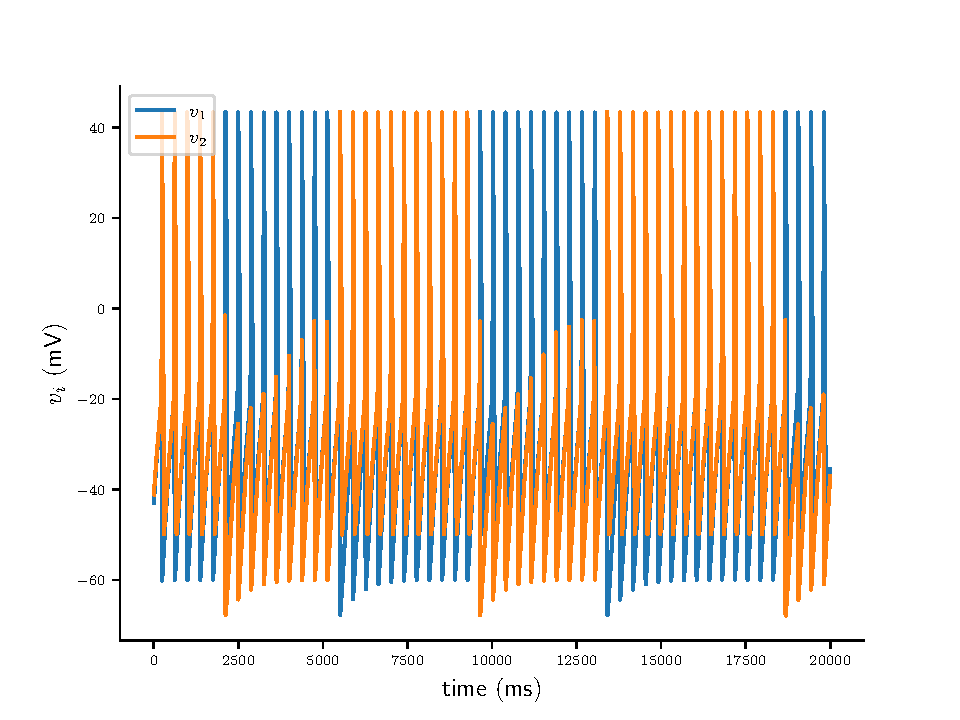
\includegraphics[width=0.7\textwidth]{irregular}
\caption{Voltage traces of an ``irregular'' solution with $\bar g=0.581$ $(\si{mS/cm^{2}})$. \label{fig:irregular}}
\end{figure}

\begin{reply}
\Cref{fig:irregular} shows an example of the aforementioned ``irregular'' solutions.
The figure was produced with strong symmetric coupling $\bar g=0.581$ $(\si{mS/cm^{2}})$, which is close to the $\bar g_{s}$ associated with the left border of the branch of suppressed solutions.
An integration time step of $dt=0.5$ $\si{ms}$ was used.
To get rid of transients the system was integrated for $500,000$ $\si{ms}$, and \cref{fig:irregular} shows the last $20,000$ $\si{ms}$.
It would be interesting to explore how chaotic the system is for large $\bar g$, but this would likely distract from the main story of the paper, which is also the main reason why we have not included this graph in the paper.
\end{reply}

\shortpoint{Page 6, line 183: The authors probably meant “fig. 4B” instead of “fig. 4A”, as the latter does not show ISI (only for the suppressed solution when it is equal to the period).}
\shortreply{Fig. 4 (M0) was removed from the paper.}

\shortpoint{Page 7, line 235: Did the authors mean ``$\bar g s$ crosses $g^{\star}$''?}
\shortreply{Corrected.}


\shortpoint{Page 7, line 246: It should be “$g^\star$” instead of “$g^*$” like throughout the manuscript.}
\shortreply{Corrected.}

\shortpoint{Page 12, line 371: It should be “is not trivial”.}
\shortreply{Corrected.}

\shortpoint{In Eq. (44) the function $G^{-1}_{n}$ cannot depend on $d^{\star}$, please revise.}
\shortreply{Indeed, thank you for spotting this. $G^{-1}_{n}$ depends on $\bar g$. Changed accordingly.}

\shortpoint{Page 13, line 383: Please remove the word “we”.}
\shortreply{Corrected.}

\shortpoint{Page 14, line 415: Ref. [21] is written twice.}
\shortreply{Corrected.}

\shortpoint{Page 17, line 511: In “Avrutin et al. and colleagues” either “et al.” or “and colleagues” should be removed.}
\shortreply{Corrected.}

\shortpoint{Fig. 1A: Marking the threshold $v_{\theta}$ would be helpful.}
\shortreply{Added $v_{\theta}$ indicators. to \cref{fig:nullclines}.}

\shortpoint{Fig. 4: The regions of overlapping (bistability) are obviously distinguishable. However, it would be helpful if they are highlighted, for instance, by vertical lines or colored vertical stripes, so that one can easier guess the approximate critical values of $\bar g$.}
\shortreply{Good idea. This will be done in the next iteration of the review process (if there is one).}

\shortpoint{Caption of Fig.10: It should be $\Pi_{n}: d^{\star}\mapsto d^{\star}$.}
\shortreply{Corrected.}


\bibliographystyle{apalike} % for Health, Physics and Mathematics articles
\bibliography{bibliography.bib}

\end{document}
